\documentclass {standalone}

\usepackage{tikz}

\begin{document}
	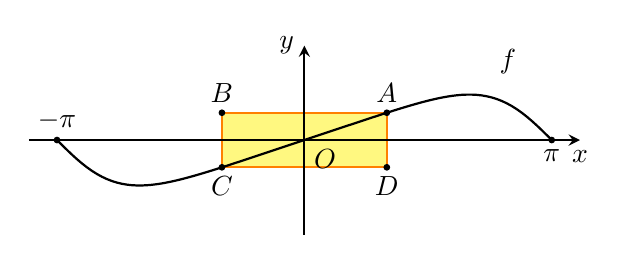
\begin{tikzpicture} [xscale=1]
		
		\coordinate (O) at (0,0);
		\coordinate (A) at (pi/3, {(sin((pi/3 r))/(2+cos(pi/3 r ))});
		\coordinate (B) at (-pi/3, {(sin((pi/3 r))/(2+cos(pi/3 r ))});
		\coordinate (C) at (-pi/3, {(sin((-pi/3 r))/(2+cos(-pi/3 r ))});
		\coordinate (D) at (pi/3, {(sin((-pi/3 r))/(2+cos(-pi/3 r ))});
	  	\coordinate (H) at (-pi,0);
	 	\coordinate (I) at (pi,0);
		
		\draw[ thick, orange, fill=yellow!50] (A) -- (B) -- (C) -- (D) -- cycle;
		
		\draw[ black, thick, domain=-pi:pi, samples=100] plot (\x, {(sin((\x r))/(2+cos(\x r )) }) ;
		
		\node[right] at ({3*pi/4},1) {$f$};			
		\node[below right] at (O)  {$O$};
		\draw[fill=black] (A) circle (1pt) node[above ]{$A$};
		\draw[fill=black] (B) circle (1pt) node[above ]{$B$};
		\draw[fill=black] (C) circle (1pt) node[below ]{$C$};
		\draw[fill=black] (D) circle (1pt) node[below ]{$D$};
		\draw[fill=black] (H) circle (1pt) node[above ]{$-\pi$};
		\draw[fill=black] (I) circle (1pt) node[below ]{$\pi$};
		\draw[->, thick, >=stealth] (-3.5,0) -- (3.5,0) node[below] {$x$};
		\draw[->, thick, >=stealth] (0,-1.2) -- (0,1.2) node[left] {$y$};
	
	\end{tikzpicture}
\end{document}
	